\chapter{真题讲解}
\label{chap22}

杭电真题只有近三年的价值最高,其他的如果时间不足可以不做☆ \newline
对应2020年考研,2017,2018,2019三年最为重要.\newline
因为有一些题目出的模棱两可,实在不必深究,这种题目会越来越少,越来越逼近408这就是趋势。\newline
注解:QU 表示此题有疑问\newline
\begin{itemize}[noitemsep,topsep=0pt,parsep=0pt,partopsep=0pt]
	\item 2017组成原理真题(150分)
	\item 2017组成原理真题答案
\end{itemize}


\section{真题}
一、判断题(对打$\checkmark$, 错打$\times$, 本大题共15小题, 每小题1分,共15分)
1. 为了提高计算机数据处理的并行能力,计算机系统结构可采用MISD结构。\newline
2. 处理器地址线的位数决定了该计算机可直接访问存储器空间的范围。\newline
3. 现代计算机由于采用多种并行处理技术,其体系结构已不是冯诺依曼体系结构。\newline
4. 十进制29的BCD码压缩型存储格式的二进制表现形式为00101010\newline
5. 八进制二进制移码11100010,其真值为十进制数-98.\newline
6. 采用三总线结构的运算器,指令ADD R0,R1 可以在一个时钟节拍内完成 (R0) + (R1) -> R0\newline
7. 浮点数加减法运算过程中,采用小阶对大阶是为了减少对阶过程中硬气的数据精度损失。\newline
8. 运算器的加减运算不见采用二进制不嘛加法器是因为不嘛运算的精度高。\newline
9. 寄存器IR是一种通用寄存器,常用来暂存数据.\newline
10. RISC系统计算机一般将使用频度高的指令采用微程序控制方式实现,而把使用频度低的指令采用硬布线方式来实现,从而尽量提高计算机的处理速度。\newline
11. 转移指令的使用会使流水线吞吐率降低。\newline
12. 先行进位加法器比行波加法器快,是因为先行进位加法器电路简单,使用门电路少,总体上降低了电路演示,从而提高了速度。\newline
13. n+1 位的证书二进制补码定义为:$$2^{n+1} + X; -2^n < x <= 2^n -1 (MOD2^{n+1})$$\newline
14. 当查找数据是,按地址访问的存储器要比按内容访问的存储器慢。相联存储器是一种按内容访问的存储器,所以查找数据较快。\newline
15. 常用的虚拟存贮系统由"主存-辅存"两级存贮器组成,其中辅存是大容量的磁表面存贮器。
二、单项选择题(请选择一个最合适的答案填入,本大题共20小题,每小题1分,共20分)
1. 若要最大限度地提高计算机并行处理能力,计算机可采用\_\_\_(1)\_\_\_结构。\newline
A. SISD                   B. SIMD
C. MISD                   D. MIMD
2. 在移码加减运算器中,采用双符号位,$S_{f1}$为高位符号位,$S_{f2}$为低符号位,则运算结果出现正溢出的情况是\_\_\_(2)\_\_\_.
A.$S_{f1}S_{f2}=00$ B.$S_{f1}S_{f2}=01$ C.$S_{f1}S_{f2}=10$ D.$S_{f1}S_{f2}=11$
3. 设机器数$[X]_{\mbox{补}}=10000000$,则X的十进制真值为\_\_\_(3)\_\_\_.
A.-0    B. 128   C. -128  D.-1
4. 数据-5的IEEE754的单精度浮点数编码为:\_\_\_(4)\_\_\_.
A. C0400000H B.CA000000H C.C0000000DH D.BF800000H
5. \_\_\_(5)\_\_\_是计算机硬件和气底层软件的特定的链接纽带。
A. 机器指令级   B.HDL语言级   C.操作系统级   D.微指令级
6.在浮点数编码表示中\_\_\_(6)\_\_\_在机器数中不出现,是隐含的。
A. 阶码  B.基数   C. 数符   D. 阶符
7.能够检出错误的校验码集的码距必需大于等于\_\_\_(7)\_\_\_
A.1    B.2   C.3   D.4
8.采用16$\times$ 16点阵显示一个汉字,其一个汉字编码需 \_\_\_(8)\_\_\_字节.
A.16 B.32  C.1  D.2
9. 下列不见中,\_\_\_(9)\_\_\_可以用来存放运算过程中的中间结果的。
A.通用寄存器 B. PC   C. CACHE   D. PSW
10. 下面存储器中,\_\_\_(10)\_\_\_的地址线通常采用分时复用的方法。
A.SRAM  B.$E^2PROM$ C. FLASH D. DRAM
11. 在普林斯顿结构的计算机中,下列叙述中不正确的是\_\_\_(11)\_\_\_。
A. 指令和数据共享一个存储器
B. 区别存储器中指令和数据的原则是根据PC去除的指令,而执行指令过程中取的是数据。
C. 指令存放在指令存储器中,数据存放在数据存储器中。
D. 采用程序存储,程序控制的方法.
12.下列编码中,有两个0的编码是\_\_\_(12)\_\_\_。
A. 反码和补码  B. 原码和补码  C.  原码和反码  D.补码和移码
13. 下面有关存储器的叙述中, \_\_\_(13)\_\_\_是错误的。
A. 采用Cache扩大了存储器的容量。
B. 双端口存储器不允许两个端口同时对同一存储单元进行写操作。
C. 采用多提交叉存储器阻止可以提高存储器的带宽。
D. DRAM是利用电容存储信息的。
14. 下面有关微指令、机器指令和微程序、程序的说法中,正确的是\_\_\_(14)\_\_\_。
A. 每一条机器指令由一段微程序解释、执行、
B. 程序是指令的有序几何,而机器指令是微程序的有序集合。
C. 微指令是一段机器指令的有序集合。
D. 微程序存放在主存中。
15. 下面关于RISC和CISC的描述中,不正确的是\_\_\_(15)\_\_\_。
A. RISC指令种类、寻址方式少、指令长度固定,所以更容易用硬布线电路实现,执行速度要比CISC快。
B. CISC的指令功能强大、寻址方式种类多,便于汇编程序员编程。
C. CISC指令种类多,所以更有利于编译、优化。
D. RISC多指令能够在一个机器周期内完成,特别适合流水线工作。
16. 下列描述中,\_\_\_(16)\_\_\_是错误的。
A. 运算器、控制器、存储器、I/O设备组成了计算机系统。
B. 运算器和控制器合在一起称CPU、
C. Von Neunanm 计算机体系结构的核心思想是存储程序、程序控制、
D.IO设备的主要作用是与计算机交换信息。
17. 若CPU需要能实时地与I/O设备交换数据并能与之并行工作,应采用\_\_\_(17)\_\_\_.
A. 程序查询方式     B.DMA方式   C. 程序中断方式     D. IO处理机方式
18. 当有中断请求信号产生时,CPU在\_\_\_(18)\_\_\_才能响应中断。
A. 当前程序执行完      B. 取指令完成   C. 当前指令执行完  D. 中断请求信号下降沿
19. 相对转移指令中转移地址的位移量采用是\_\_\_(19)\_\_\_表示。
A. 无符号二进制数   B. 原码  C. 补码  D. 移码
20. 某机采用三级流水线阻止,分别为取指令译码、计算地址、执行阶段。一部分指令取指令译码需要在$t_1$时间完成,另一些指令需要$t_4$时间完成;计算地址一部分指令需要$t_2$时间完成, 另一些指令需要$t_5$时间餐能完成;执行阶段一部分需要$t_3$时间完成,另一些指令需要$t_6$时间完成,则机器周期T应选\_\_\_(20)\_\_\_。
A. T=min($t_1,t_2,t_3,t_4,t_5,t_6$)   B. T=$t_4$    
C. ($t_1+t_2+t_3+t_4+t_5+t_6$) / 6  D. T=max($t_1+t_2+t_3+t_4+t_5+t_6$)

三、简答题(本大题共5小题, 每小题5分, 共25分)
1. 写出阶码6位(包含以为符号位)、尾数10位(包含一位符号位)、阶码和尾数均用补码表示的16位规格化浮点数能表示的最大数、最小数、最小正数、最大负数及机器零。
2. 请说出相联存储器在Cache地址映射中的作用。
3. 在控制器控制方式中,一部控制与联合控制有什么区别?
4. 虚拟存储器的目的是什么?逻辑地址转换为物理地址有哪些方法?
5. 说明RISC和CISC指令系统的区别。
四、填空题(本大题共25空,每空1分,共25分; 请按照小标好(1) ~ (25) 顺序答题)
1. DRAM 有三种刷新方式,分别是\_\_\_(1)\_\_\,\_\_\_(2)\_\_\,\_\_\_(3)\_\_\.
2. 在多体交叉阻止的存储器系统中,存储器地址编码方式是: 地址的高若干位部分用作为\_\_\_(4)\_\_\ ,而地址的低若干用作\_\_\_(5)\_\_\ 。
3. 设X=-110100,则8位机器数$[X]_{\mbox{原}}=$ \_\_\_(6)\_\_\ ,$[X]_{\mbox{反}}=$\_\_\_(7)\_\_\ ,$[X]_{\mbox{补}}=$\_\_\_(8)\_\_\ ,$[X]_{\mbox{移}}=$\_\_\_(9)\_\_\ ,$[X/2]_{\mbox{补}}=$\_\_\_(10)\_\_\ .
4. 设寄存器RO=0A5H, 变址寄存器SI=30H,在地址33H单元存放了0D6H,在执行了指令"SUB R0, [SI+3]"后(R0为目的操作数),则寄存器R0的内容=\_\_\_(11)\_\_\, 标志寄存器CF=\_\_\_(12)\_\_\ ; OF=\_\_\_(13)\_\_\ ; ZF=\_\_\_(14)\_\_\ ; SF=\_\_\_(15)\_\_\ , 该指令内存数据采用的寻址方式是:\_\_\_(16)\_\_\ .
5. 设在穿行数据通讯中, 数据位8位, 采用奇校验码, 如果收到的8位为01101101,则表示收到的数据是对的吗? 答: \_\_\_(17)\_\_\
6. 设有$[X]_{补}=X_0 X_1 X_2...X_N$,$[Y]_{\mbox{补}}=Y_0,Y_1Y_2..Y_n$,在补码乘法Booth算法运算过程中,$Y_{n+1}$必需等于\_\_\_(18)\_\_\_,
$Y_{i+1}-Y_{i}=0$,则需\_\_\_(19)\_\_\_,然后部分积连同乘数右移一位,若$Y_{i+1}-Y_{i}=-1$,则需\_\_\_(20)\_\_\_,然后部分积连同乘数右移一位。\newline
7. 微机A、B是采用不同主频的CPU芯片,片内逻辑电路完全相同,若A机的CPU主频为4MHZ,B机为12MH。A机的品骏指令执行速度为0.5MIPS,那么A机的平均指令周期为\_\_\_(21)\_\_\_us,B机的平均指令执行速度为\_\_\_(22)\_\_\_MIPS。\newline
8.在控制器中,IR用于存放\_\_\_(23)\_\_\_.\newline
9.在微程序控制的计算机中,指令译码器的作用是\_\_\_(24)\_\_\_,一条机器指令的执行实际上就是执行一端存放在\_\_\_(25)\_\_\_中的微程序。
五、计算题(本大题共2题,共30分)\newline
1. (本题每空2分,共16分)设8位计算机主存容量为64K,存储器按字节编织,Cache容量为256字节,每块4字节,Cache按2路组相联方式组织,则主存地址至少需\_\_\_(1)\_\_\_,其中“标记”字段\_\_\_(2)\_\_\_位,Cache组地址\_\_\_(3)\_\_\_,块内地址\_\_\_(4)\_\_\_位,主存地址285EH可映射到Cache的第\_\_\_(5)\_\_\_组。设CPU总是从Cache取得数据,一直Cache的存储周期为5ns,主存的存储周期为50ns。设下列指令都是2字节的指令,若在执行系列程序之前Cache为空,则执行下列程序后:\newline
       ORG    000H\newline
START: MOV    R0,#50 ;50 -> R0\newline
       MOV    R1,#0\newline
       MOV    R2,#0\newline
LOOP1: ADD    R1,R0; (R1) + (R0) -> R1\newline
       ADC    R2,#0; (R2) +CY(进位) ->R2\newline
       SUB    R0,#1;\newline
       JNE    LOOP1\newline
       HLAT\newline
问Cache的命中率为\_\_\_(6)\_\_\_,Cache/主存的平均访问时间为\_\_\_(7)\_\_\_ns,Cache/主存的效率为\_\_\_(8)\_\_\_。\newline
2.(本题共14分)设浮点数的格式为:阶码5位,包含一位符号位,尾数8位,包含一位符号位,阶码和尾数军用补码表示,排列顺序为:\newline
\begin{center}
	\begin{tabular}{|c|c|c|c|}% 通过添加 | 来表示是否需要绘制竖线
		\hline  % 在表格最上方绘制横线
		阶符(1位)   & 阶码(4位) & 数符(1位) & 尾数(7位)\\
		\hline  %在第一行和第二行之间绘制横线
	\end{tabular}
\end{center}
(1)(本小题4分)假设$(X)_{10} = -23/256$,则按上述浮点数的格式:写出X的规格化浮点数表示形式;\newline
(2)(本小题10分)设$[X]_{\mbox{浮}=0,0010  1.0100101, [Y]_{\mbox{浮}}=0,0101 0.010 1100}$用浮点数计算$[X+Y]_{\mbox{浮}}$,请写出每一步计算过程。\newline
六、综合设计题(本大题共3题,共35分)
1.(本题10分)设CPU有地址线$A_{19}~A_{0}$,数据线$D_{15}~D_{0}$,读写信号线WE#(低电平写,高电平读),存储请求线MREQ#(低电平有效)等,若CPU与2篇8K$\times$16bit和4片16K$\times$8bit的SRAM组成的48K$\times$16bit的存储器系统,SRAM存储器芯片除地址线和数据线外,还有CS#为芯片选择信号(低电平有效),R/W#为读写信号(高电平为读,低电平为写),8KW的SRAM地址从F2000H开始占有16K为连续地址空间,16KB的SRAM地址从F8000H开始占有连续的32K地址空间,若采用3-8译码器和一些门电路器件,画出CPU与存储器的连接图(要求画出具体的译码电路,标出连接的数据线和地址线的位数、使用的信号线名称等)。\newline
2.(本题15分)设某8位计算机结构图如图1所示,每个信号的下标in表示数据从总线到部件的输入控制信号,out表示数据从部件输出到总线的控制信号,所有的微命令信号已在图上标出,采用微程序设计技术,要求:\newline
(1)(本小题7分)试列表将所有信号按照互斥命令归类分组,哪组型号是电平信号,哪组是边沿触发的控制信号?\newline
(2)(本小题8分)画出实现指令ADD  R0,[SI+05]的微指令流程图。\newline
\begin{figure}[H]
	\centering  % 环境中的内容居中排版
	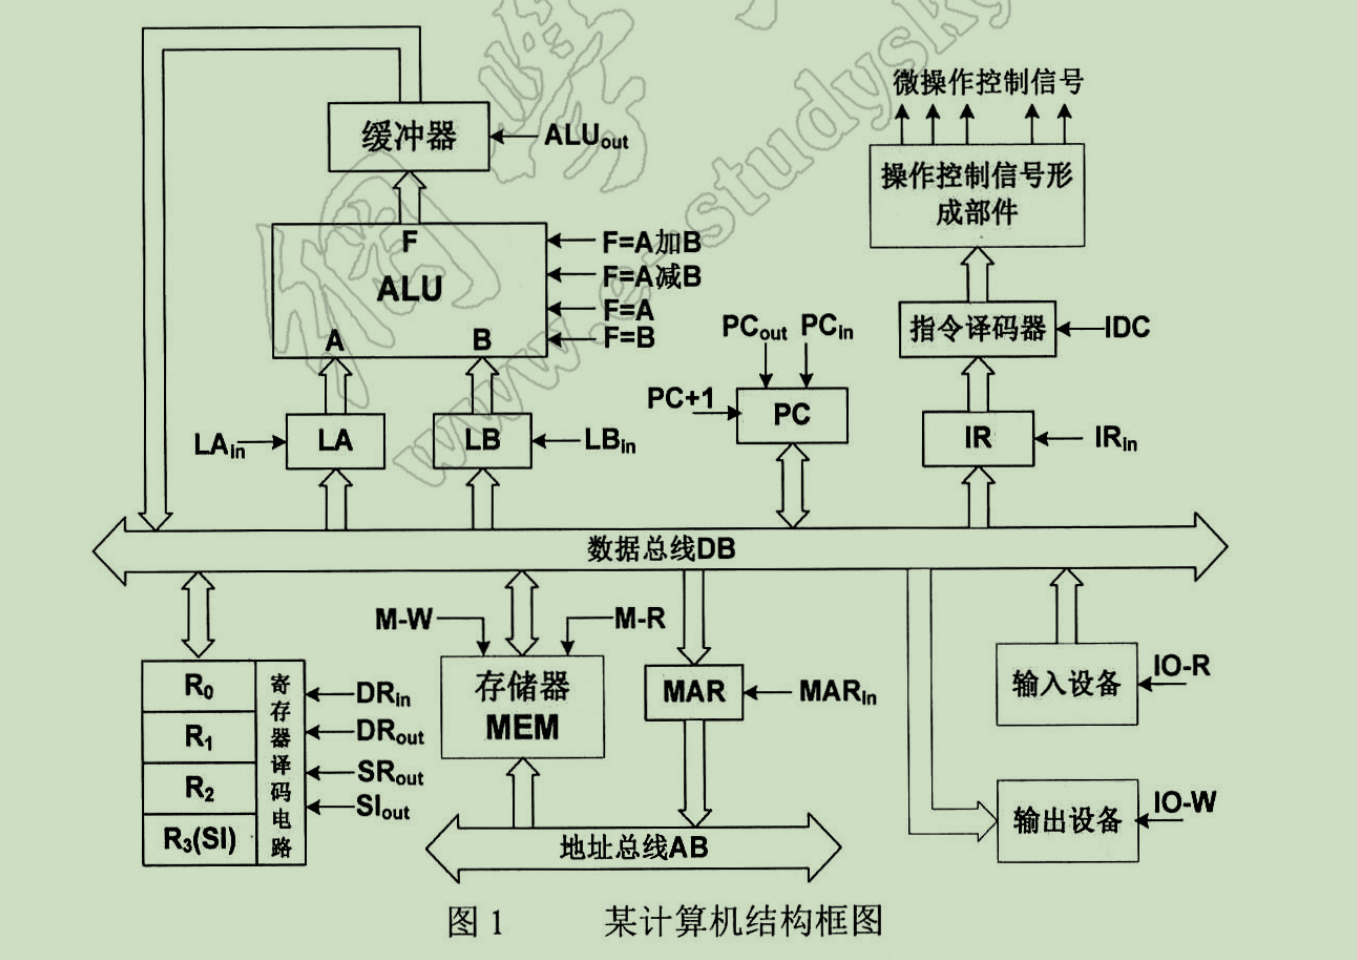
\includegraphics[scale=0.3]{example/chapter22/2019-11-12145424.png}
\end{figure}
3.(本题10分)图2是MIPS的一种指令结构图。\newline
(1)(本小题6分)请描述指令 ADD \$S0,\$T0,\$T1的指令过程和数据通路(寄存器T0的内容加上寄存器T1的内容结果送到寄存器S0中)。\newline
(2)(本小题2分)该指令是什么类型的指令结构?\newline
(3)(本小题2分)该指令的执行最少需要几个时钟周期?\newline
\begin{figure}[H]
	\centering  % 环境中的内容居中排版
	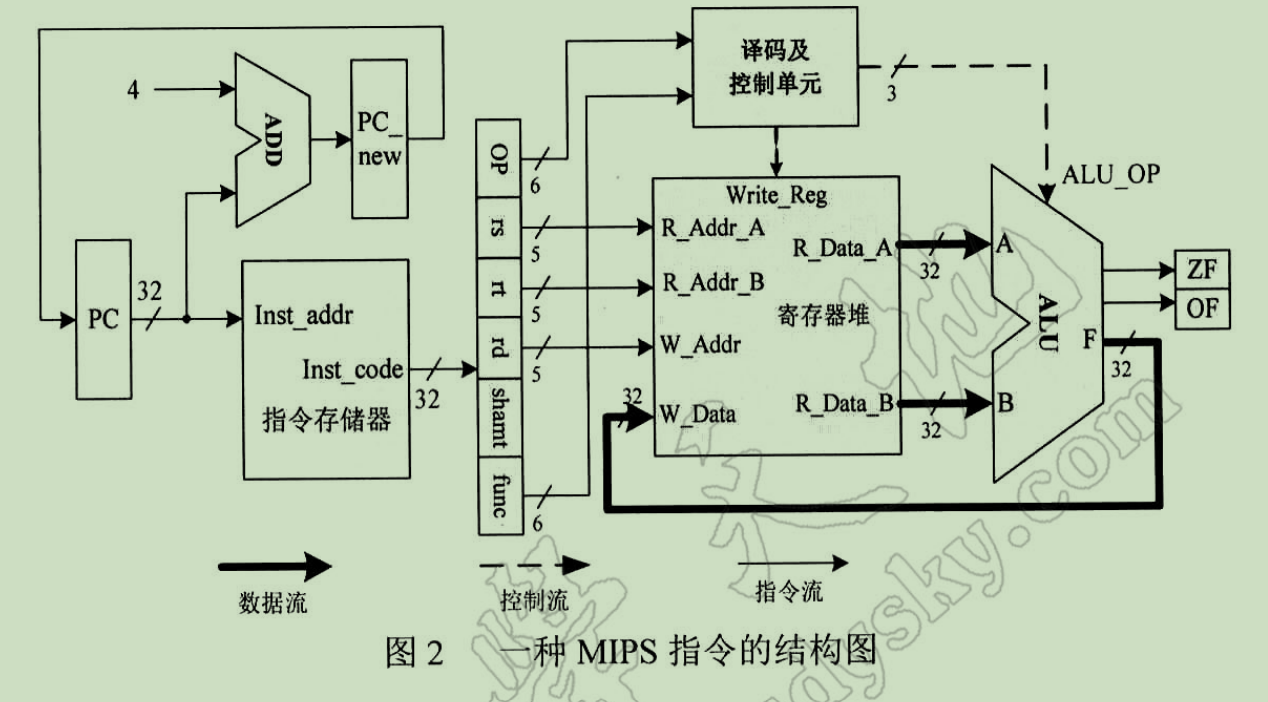
\includegraphics[scale=0.3]{example/chapter22/2019-11-12152727.png}
\end{figure}



TIPS:冯.诺伊曼体系结构是现代计算机的基础,现在大多计算机仍是冯.诺伊曼计算机的组织结构,只是作了一些改进而已,并没有从根本上突破冯体系结构的束缚。

\section{答案}
一、判断题(对打$\checkmark$, 错打$\times$, 本大题共15小题, 每小题1分,共15分)
1. 为了提高计算机数据处理的并行能力,计算机系统结构可采用MISD结构。\newline
解:$\times$,并行处理能力是MIMD,多指令流,多数据流\newline
2. 处理器地址线的位数决定了该计算机可直接访问存储器空间的范围。\newline
解:$ \checkmark $\newline
3. 现代计算机由于采用多种并行处理技术,其体系结构已不是冯诺依曼体系结构。\newline
解:$  \checkmark  $,早期采用的是以控制器为中心的结构,现在采用的是以存储器为中心的结构\newline
4. 十进制29的BCD码压缩型存储格式的二进制表现形式为00101010\newline
解:$  \checkmark  $压缩性还是非压缩性参考链接 https://zhidao.baidu.com/question/71096441.html , 所以是正确的压缩型采用的是一个字节存放两个BCD数字。\newline
5. 八进制二进制移码11100010,其真值为十进制数-98.\newline
解:$\times$移码转为补码为01100010,因为补码是正数所以十进制数不可能是负数。\newline
6. 采用三总线结构的运算器,指令ADD R0,R1 可以在一个时钟节拍内完成 (R0) + (R1) -> R0\newline
解:$\checkmark$,寻找三总线结构的结构图即可知。\newline 
7. 浮点数加减法运算过程中,采用小阶对大阶是为了减少对阶过程中引起的数据精度损失。\newline
解:$\checkmark$ ,参考链接https://zhidao.baidu.com/question/543978375.html\newline
8. 运算器的加减运算部件采用二进制补码加法器是因为补码运算的精度高。\newline
解:$\times$,因为减法也能采用加法模拟\newline
9. 寄存器IR是一种通用寄存器,常用来暂存数据.\newline
解:$\times$,IR是指令寄存器,不是通用寄存器,AC才是通用寄存器。
10. RISC系统计算机一般将使用频度高的指令采用微程序控制方式实现,而把使用频度低的指令采用硬布线方式来实现,从而尽量提高计算机的处理速度。\newline
解:$\times$,RISC是精简指令集,所以以硬布线的方式为主。
11. 转移指令的使用会使流水线吞吐率降低。\newline
解:$\checkmark$,正确,流水线会重新开始流动。
12. 先行进位加法器比行波加法器快,是因为先行进位加法器电路简单,使用门电路少,总体上降低了电路演示,从而提高了速度。\newline
解:?
13. n+1 位的整数二进制补码定义为:$$2^{n+1} + X; -2^n < x <= 2^n -1 (MOD2^{n+1})$$\newline
解:?
14. 当查找数据是,按地址访问的存储器要比按内容访问的存储器慢。相联存储器是一种按内容访问的存储器,所以查找数据较快。\newline
解:?
15. 常用的虚拟存贮系统由"主存-辅存"两级存贮器组成,其中辅存是大容量的磁表面存贮器。\newline
解:$\checkmark$\newline
二、单项选择题(请选择一个最合适的答案填入,本大题共20小题,每小题1分,共20分)
1. 若要最大限度地提高计算机并行处理能力,计算机可采用\_\_\_(1)\_\_\_结构。\newline
A. SISD                   B. SIMD
C. MISD                   D. MIMD
解:D\newline
2. 在移码加减运算器中,采用双符号位,$S_{f1}$为高位符号位,$S_{f2}$为低符号位,则运算结果出现正溢出的情况是\_\_\_(2)\_\_\_.
A.$S_{f1}S_{f2}=00$ B.$S_{f1}S_{f2}=01$ C.$S_{f1}S_{f2}=10$ D.$S_{f1}S_{f2}=11$
解:?
3. 设机器数$[X]_{\mbox{补}}=10000000$,则X的十进制真值为\_\_\_(3)\_\_\_.
A.-0    B. 128   C. -128  D.-1
解:C, -128的补码为10000000\newline
4. 数据-5的IEEE754的单精度浮点数编码为:\_\_\_(4)\_\_\_.
A. C0400000H B.CA000000H C.C0000000DH D.BF800000H
解:?
5. \_\_\_(5)\_\_\_是计算机硬件和其底层软件的特定的链接纽带。
A. 机器指令级   B.HDL语言级   C.操作系统级   D.微指令级
解:A\newline
6.在浮点数编码表示中\_\_\_(6)\_\_\_在机器数中不出现,是隐含的。
A. 阶码  B.基数   C. 数符   D. 阶符
解:B\newline
7.能够检出错误的校验码集的码距必需大于等于\_\_\_(7)\_\_\_
A.1    B.2   C.3   D.4
解:B\newline
8.采用16$\times$ 16点阵显示一个汉字,其一个汉字编码需 \_\_\_(8)\_\_\_字节.
A.16 B.32  C.1  D.2
解:B 16*16 / 8 = 32字节\newline
9. 下列部件中,\_\_\_(9)\_\_\_可以用来存放运算过程中的中间结果的。
A.通用寄存器 B. PC   C. CACHE   D. PSW
解:A
10. 下面存储器中,\_\_\_(10)\_\_\_的地址线通常采用分时复用的方法。
A.SRAM  B.$E^2PROM$ C. FLASH D. DRAM
解:D
11. 在普林斯顿结构的计算机中,下列叙述中不正确的是\_\_\_(11)\_\_\_。
A. 指令和数据共享一个存储器
B. 区别存储器中指令和数据的原则是根据PC去除的指令,而执行指令过程中取的是数据。
C. 指令存放在指令存储器中,数据存放在数据存储器中。
D. 采用程序存储,程序控制的方法.
解:C不准确,因为C是哈弗的特点.
12.下列编码中,有两个0的编码是\_\_\_(12)\_\_\_。
A. 反码和补码  B. 原码和补码  C.  原码和反码  D.补码和移码
解:C\newline
13. 下面有关存储器的叙述中, \_\_\_(13)\_\_\_是错误的。
A. 采用Cache扩大了存储器的容量。
B. 双端口存储器不允许两个端口同时对同一存储单元进行写操作。
C. 采用多体交叉存储器阻止可以提高存储器的带宽。
D. DRAM是利用电容存储信息的。
解:A,没有扩大,只是加快了数据的存储 \newline 
14. 下面有关微指令、机器指令和微程序、程序的说法中,正确的是\_\_\_(14)\_\_\_。
A. 每一条机器指令由一段微程序解释、执行。
B. 程序是指令的有序集合,而机器指令是微程序的有序集合。
C. 微指令是一段机器指令的有序集合。
D. 微程序存放在主存中。
解:A  
15. 下面关于RISC和CISC的描述中,不正确的是\_\_\_(15)\_\_\_。
A. RISC指令种类、寻址方式少、指令长度固定,所以更容易用硬布线电路实现,执行速度要比CISC快。
B. CISC的指令功能强大、寻址方式种类多,便于汇编程序员编程。
C. CISC指令种类多,所以更有利于编译、优化。
D. RISC多指令能够在一个机器周期内完成,特别适合流水线工作。
解: C  不利于编译优化
16. 下列描述中,\_\_\_(16)\_\_\_是错误的。
A. 运算器、控制器、存储器、I/O设备组成了计算机系统。
B. 运算器和控制器合在一起称CPU、
C. Von Neunanm 计算机体系结构的核心思想是存储程序、程序控制、
D. IO设备的主要作用是与计算机交换信息。
解:A 计算机由控制器、运算器、存储器、输入设备、输出设备五部分组成,而不是计算机系统
17. 若CPU需要能实时地与I/O设备交换数据并能与之并行工作,应采用\_\_\_(17)\_\_\_.
A. 程序查询方式     B.DMA方式   C. 程序中断方式     D. IO处理机方式
解:D ??????
18. 当有中断请求信号产生时,CPU在\_\_\_(18)\_\_\_才能响应中断。
A. 当前程序执行完      B. 取指令完成   C. 当前指令执行完  D. 中断请求信号下降沿
解:C
19. 相对转移指令中转移地址的位移量采用是\_\_\_(19)\_\_\_表示。
A. 无符号二进制数   B. 原码  C. 补码  D. 移码
解: C 计算机中的大部分运算都是补码
20. 某机采用三级流水线阻止,分别为取指令译码、计算地址、执行阶段。一部分指令取指令译码需要在$t_1$时间完成,另一些指令需要$t_4$时间完成;计算地址一部分指令需要$t_2$时间完成, 另一些指令需要$t_5$时间餐能完成;执行阶段一部分需要$t_3$时间完成,另一些指令需要$t_6$时间完成,则机器周期T应选\_\_\_(20)\_\_\_。
A. T=min($t_1,t_2,t_3,t_4,t_5,t_6$)   B. T=$t_4$    
C. ($t_1+t_2+t_3+t_4+t_5+t_6$) / 6  D. T=max($t_1+t_2+t_3+t_4+t_5+t_6$)
解:D 机器周期选择最大的时间。


三、简答题(本大题共5小题, 每小题5分, 共25分)
1. 写出阶码6位(包含以为符号位)、尾数10位(包含一位符号位)、阶码和尾数均用补码表示的16位规格化浮点数能表示的最大数、最小数、最小正数、最大负数及机器零。
解:??
2. 请说出相联存储器在Cache地址映射中的作用。
解:??
3. 在控制器控制方式中,异步控制与联合控制有什么区别?
解:\newline
异步控制方式:每个微操作的时钟周期个数可能不同。控制器的电路比较复杂。\newline
联合控制方式:把同步控制和异步控制结合起来,思想是,在功能部件内部采用同步控制方式,在功能部件之间采用异步控制方式。能保证一定的速度,控制电路设计相对复杂。
同步控制方式:控制器产生统一的、顺序固定的,周而复始的节拍电位(机器周期信号)和节拍脉冲(时钟周期信号),电路简单,运行速度慢。
4. 虚拟存储器的目的是什么?逻辑地址转换为物理地址有哪些方法?
5. 说明RISC和CISC指令系统的区别。



















